\newcommand{\setup}[2]{
%----------------------------------------------------------------------------------------
%	PACKAGES AND OTHER DOCUMENT CONFIGURATIONS
%----------------------------------------------------------------------------------------

    \documentclass[a4paper, 11pt, oneside]{book} % A4 paper size, default 11pt font size and oneside for equal margins

    \usepackage[margin=1in,nomarginpar]{geometry}
    \usepackage[utf8]{inputenc} % Required for inputting international characters
    \usepackage[T1]{fontenc} % Output font encoding for international characters
    \usepackage{fouriernc} % Use the New Century Schoolbook font
    \usepackage{titletoc}% http://ctan.org/pkg/titletoc
    \usepackage{hyperref}
    \usepackage{graphicx}
    \usepackage{lipsum}
    \usepackage{caption}
    \usepackage{float}
    \usepackage{amssymb}
    \usepackage{amsmath}

    \usepackage{xlop}
    \usepackage{tikz}
    \usepackage{xfp}
    \usepackage{soul}
    \usepackage{xifthen}
    \sodef\carrystyle{}{0.45em}{0em}{-0.25em}

    \newcommand{\opandbin}[3]{
        \oplogicalbin{##1}{##2}{##3}{$\land$}
    }

    \newcommand{\oporbin}[3]{
        \oplogicalbin{##1}{##2}{##3}{$\lor$}
    }

    \newcommand{\oplogicalbin}[4] {
        \begin{tabular}[t]{rr}
            &\pgfmathbin{##1}\pgfmathresult\\
            ##4&\pgfmathbin{##2}\pgfmathresult\\\hline
            &\pgfmathbin{##3}\pgfmathresult
        \end{tabular}
    }

    \newcommand{\opaddbin}[3]{
        \newcommand{\resultInBaseTen}{\fpeval{##1+##2}}

        \newcount\currentValue
        \newcount\basenumberlength
        \currentValue=\resultInBaseTen
        \basenumberlength=0

        \loop
        \advance \basenumberlength + 1
        \currentValue=\numexpr \currentValue / 2\relax
        \ifnum \currentValue > 1
        \repeat

        \pgfmathsetbasenumberlength{\basenumberlength}
        \begin{tabular}[t]{rr}
            \ifthenelse{\isempty{##3}}%
            {}% if #3 is empty
            {&\pgfcarrybin{##3}\\}% if #3 is not empty
            &\pgfmathbin{##1}\pgfmathresult\\
            +&\pgfmathbin{##2}\pgfmathresult\\\hline
            &\pgfmathbin{\resultInBaseTen}\pgfmathresult
        \end{tabular}
    }

    \newcommand{\pgfcarry}[1]{
        \begin{tiny}
            \expandafter\carrystyle\expandafter{##1}
        \end{tiny}
    }

    \newcommand{\pgfcarrybin}[1] {
        \pgfmathbin{##1}
        \pgfcarry{\pgfmathresult}
    }

    \usepackage{a4wide}
    \usepackage[#1]{babel}
    \usepackage[#2]{csquotes}
    \newcommand*{\itenquote}[1]{\enquote{{\itshape##1}}}
    \newcommand{\para}{\\[12pt]}
    \usepackage{subcaption}
    \usepackage[]{algorithm2e}
    \usepackage[local,nolabels,exerciseaslist,usesolutionserieslabels]{exsol}
    \renewcommand{\loadSolutions}{
        \immediate\closeout\solutionstream
        \input{\jobname.sol.tex}
        \immediate\openout\solutionstream=\jobname.sol.tex
    }

    \setlength{\exsolexercisetopbottomsep}{0pt plus 0pt minus 1pt}
    \setlength{\exsolexerciseleftmargin}{2em}
    \setlength{\exsolexerciserightmargin}{1em}
    \setlength{\exsolexerciseparindent}{0em}
    \setlength{\exsolexerciselabelsep}{1ex}
    \setlength{\exsolexerciselabelwidth}{30pt}
    \setlength{\exsolexerciseitemindent}{0pt}
    \setlength{\exsolexerciseparsep}{\parskip}

    \usepackage[postpunc={dot},% full stop after description
    nostyles,% don't load default style packages
% load glossaries-extra-stylemods.sty and glossary-tree.sty:
    stylemods={tree}
    ]{glossaries-extra}

    \usepackage[backend=biber,
    style=alphabetic,
    ]{biblatex}

    \usepackage[nottoc]{tocbibind}
    \usepackage{listings}
    \usepackage{xcolor}

    \colorlet{punct}{red!60!black}
    \definecolor{background}{HTML}{EEEEEE}
    \definecolor{delim}{RGB}{20,105,176}
    \colorlet{numb}{magenta!60!black}

    \lstdefinelanguage{json}{
        basicstyle=\normalfont\ttfamily,
        numbers=left,
        numberstyle=\scriptsize,
        stepnumber=1,
        numbersep=8pt,
        showstringspaces=false,
        breaklines=true,
        frame=lines,
        backgroundcolor=\color{background},
        literate=
        *{0}{{{\color{numb}0}}}{1}
        {1}{{{\color{numb}1}}}{1}
        {2}{{{\color{numb}2}}}{1}
        {3}{{{\color{numb}3}}}{1}
        {4}{{{\color{numb}4}}}{1}
        {5}{{{\color{numb}5}}}{1}
        {6}{{{\color{numb}6}}}{1}
        {7}{{{\color{numb}7}}}{1}
        {8}{{{\color{numb}8}}}{1}
        {9}{{{\color{numb}9}}}{1}
        {:}{{{\color{punct}{:}}}}{1}
        {,}{{{\color{punct}{,}}}}{1}
        {\{}{{{\color{delim}{\{}}}}{1}
        {\}}{{{\color{delim}{\}}}}}{1}
        {[}{{{\color{delim}{[}}}}{1}
        {]}{{{\color{delim}{]}}}}{1},
}

% Table of contents with links
\hypersetup{
colorlinks,
citecolor=black,
filecolor=black,
linkcolor=black,
urlcolor=black
}
}
\setup{ngerman}{german=swiss}

% glossary
\newglossaryentry{GAN} {
    name = {GAN},
    description = {Generative Adversarial Networks - Zwei neuronale Netze, die ein Nullsummenspiel durchführen.
    Eines erstellt Kandidaten, das andere bewertet sie.\cite{wiki:gan}}
}
\newglossaryentry{Multilayer perceptron} {
    name = {Multilayer-Perceptron},
    plural = {Multilayer-Perceptronen},
    description = {Ein Multilayer-Perceptron ist eine Klasse von künstlichen neuronalen Netzen. Es besteht aus mindestens
    drei Layern: dem Input-Layer, einem Hidden-Layer und einem Output-Layer. Vielfach wird es auch als \glqq vanilla\grqq{}
        neuronales Netz bezeichnet.\cite{wiki:multilayerPerceptron}}
}
\newglossaryentry{KNN} {
    name = {KNN},
    description = {Siehe \Gls{Multilayer perceptron}}
}
\newglossaryentry{Backpropagation} {
    name = {Backpropagation},
    description = {Die Backpropagation beschreibt ein Verfahren, um neuronale Netze zu trainieren. Es basiert auf dem
    mittleren quadratischen Fehler und gehört zu der Gruppe der überwachten Lernverfahren.\cite{wiki:backpropagation}}
}
\newglossaryentry{CNN} {
    name = {Convolutional Neuronal Network},
    description = {Dabei handelt es sich um eine spezielle Architektur eines \Gls{KNN}. Es funktioniert nach dem Prinzip
        der Konvolution. Das heisst, die Gewichte auf den Kanten sind nicht flach, diese werden über Konvolutions-Filter
        definiert und viele Bildabschnitte teilen sich so die Gewichte.\cite{wiki:cnn}}
}

\addbibresource{../common/resources/literature.bib}

\begin{document}

    %%%%%%%%%%%%%%%%%%%%%%%%%%%%%%%%%%%%%%%%%
% Formal Book Title Page
% LaTeX Template
% Version 2.0 (23/7/17)
%
% This template was downloaded from:
% http://www.LaTeXTemplates.com
%
% Original author:
% Peter Wilson (herries.press@earthlink.net) with modifications by:
% Vel (vel@latextemplates.com)
%
% License:
% CC BY-NC-SA 3.0 (http://creativecommons.org/licenses/by-nc-sa/3.0/)
%
% This template can be used in one of two ways:
%
% 1) Content can be added at the end of this file just before the \end{document}
% to use this title page as the starting point for your document.
%
% 2) Alternatively, if you already have a document which you wish to add this
% title page to, copy everything between the \begin{document} and
% \end{document} and paste it where you would like the title page in your
% document. You will then need to insert the packages and document
% configurations into your document carefully making sure you are not loading
% the same package twice and that there are no clashes.
%
%%%%%%%%%%%%%%%%%%%%%%%%%%%%%%%%%%%%%%%%%

%----------------------------------------------------------------------------------------
%	TITLE PAGE
%----------------------------------------------------------------------------------------

\begin{titlepage} % Suppresses headers and footers on the title page

	\centering % Centre everything on the title page

	\scshape % Use small caps for all text on the title page

	\vspace*{\baselineskip} % White space at the top of the page

	%------------------------------------------------
	%	Title
	%------------------------------------------------

	\rule{\textwidth}{1.6pt}\vspace*{-\baselineskip}\vspace*{2pt} % Thick horizontal rule
	\rule{\textwidth}{0.4pt} % Thin horizontal rule

	\vspace{0.75\baselineskip} % Whitespace above the title

	{\LARGE GAN - Generative Adversarial Networks\\} % Title

	\vspace{0.75\baselineskip} % Whitespace below the title

	\rule{\textwidth}{0.4pt}\vspace*{-\baselineskip}\vspace{3.2pt} % Thin horizontal rule
	\rule{\textwidth}{1.6pt} % Thick horizontal rule

	\vspace{2\baselineskip} % Whitespace after the title block

	%------------------------------------------------
	%	Subtitle
	%------------------------------------------------

	Eine weitere Architektur % Subtitle or further description

	\vspace*{3\baselineskip} % Whitespace under the subtitle

	%------------------------------------------------
	%	Editor(s)
	%------------------------------------------------

	Von

	\vspace{0.5\baselineskip} % Whitespace before the editors

	{\scshape\Large Luca Ritz} % Editor list

	\vspace{0.5\baselineskip} % Whitespace below the editor list

	\textit{BFH - Berner Fachhochschule} % Editor affiliation

	\vfill % Whitespace between editor names and publisher logo

	%------------------------------------------------
	%	Publisher
	%------------------------------------------------

	\begin{figure}[h!]
		\begin{center}
			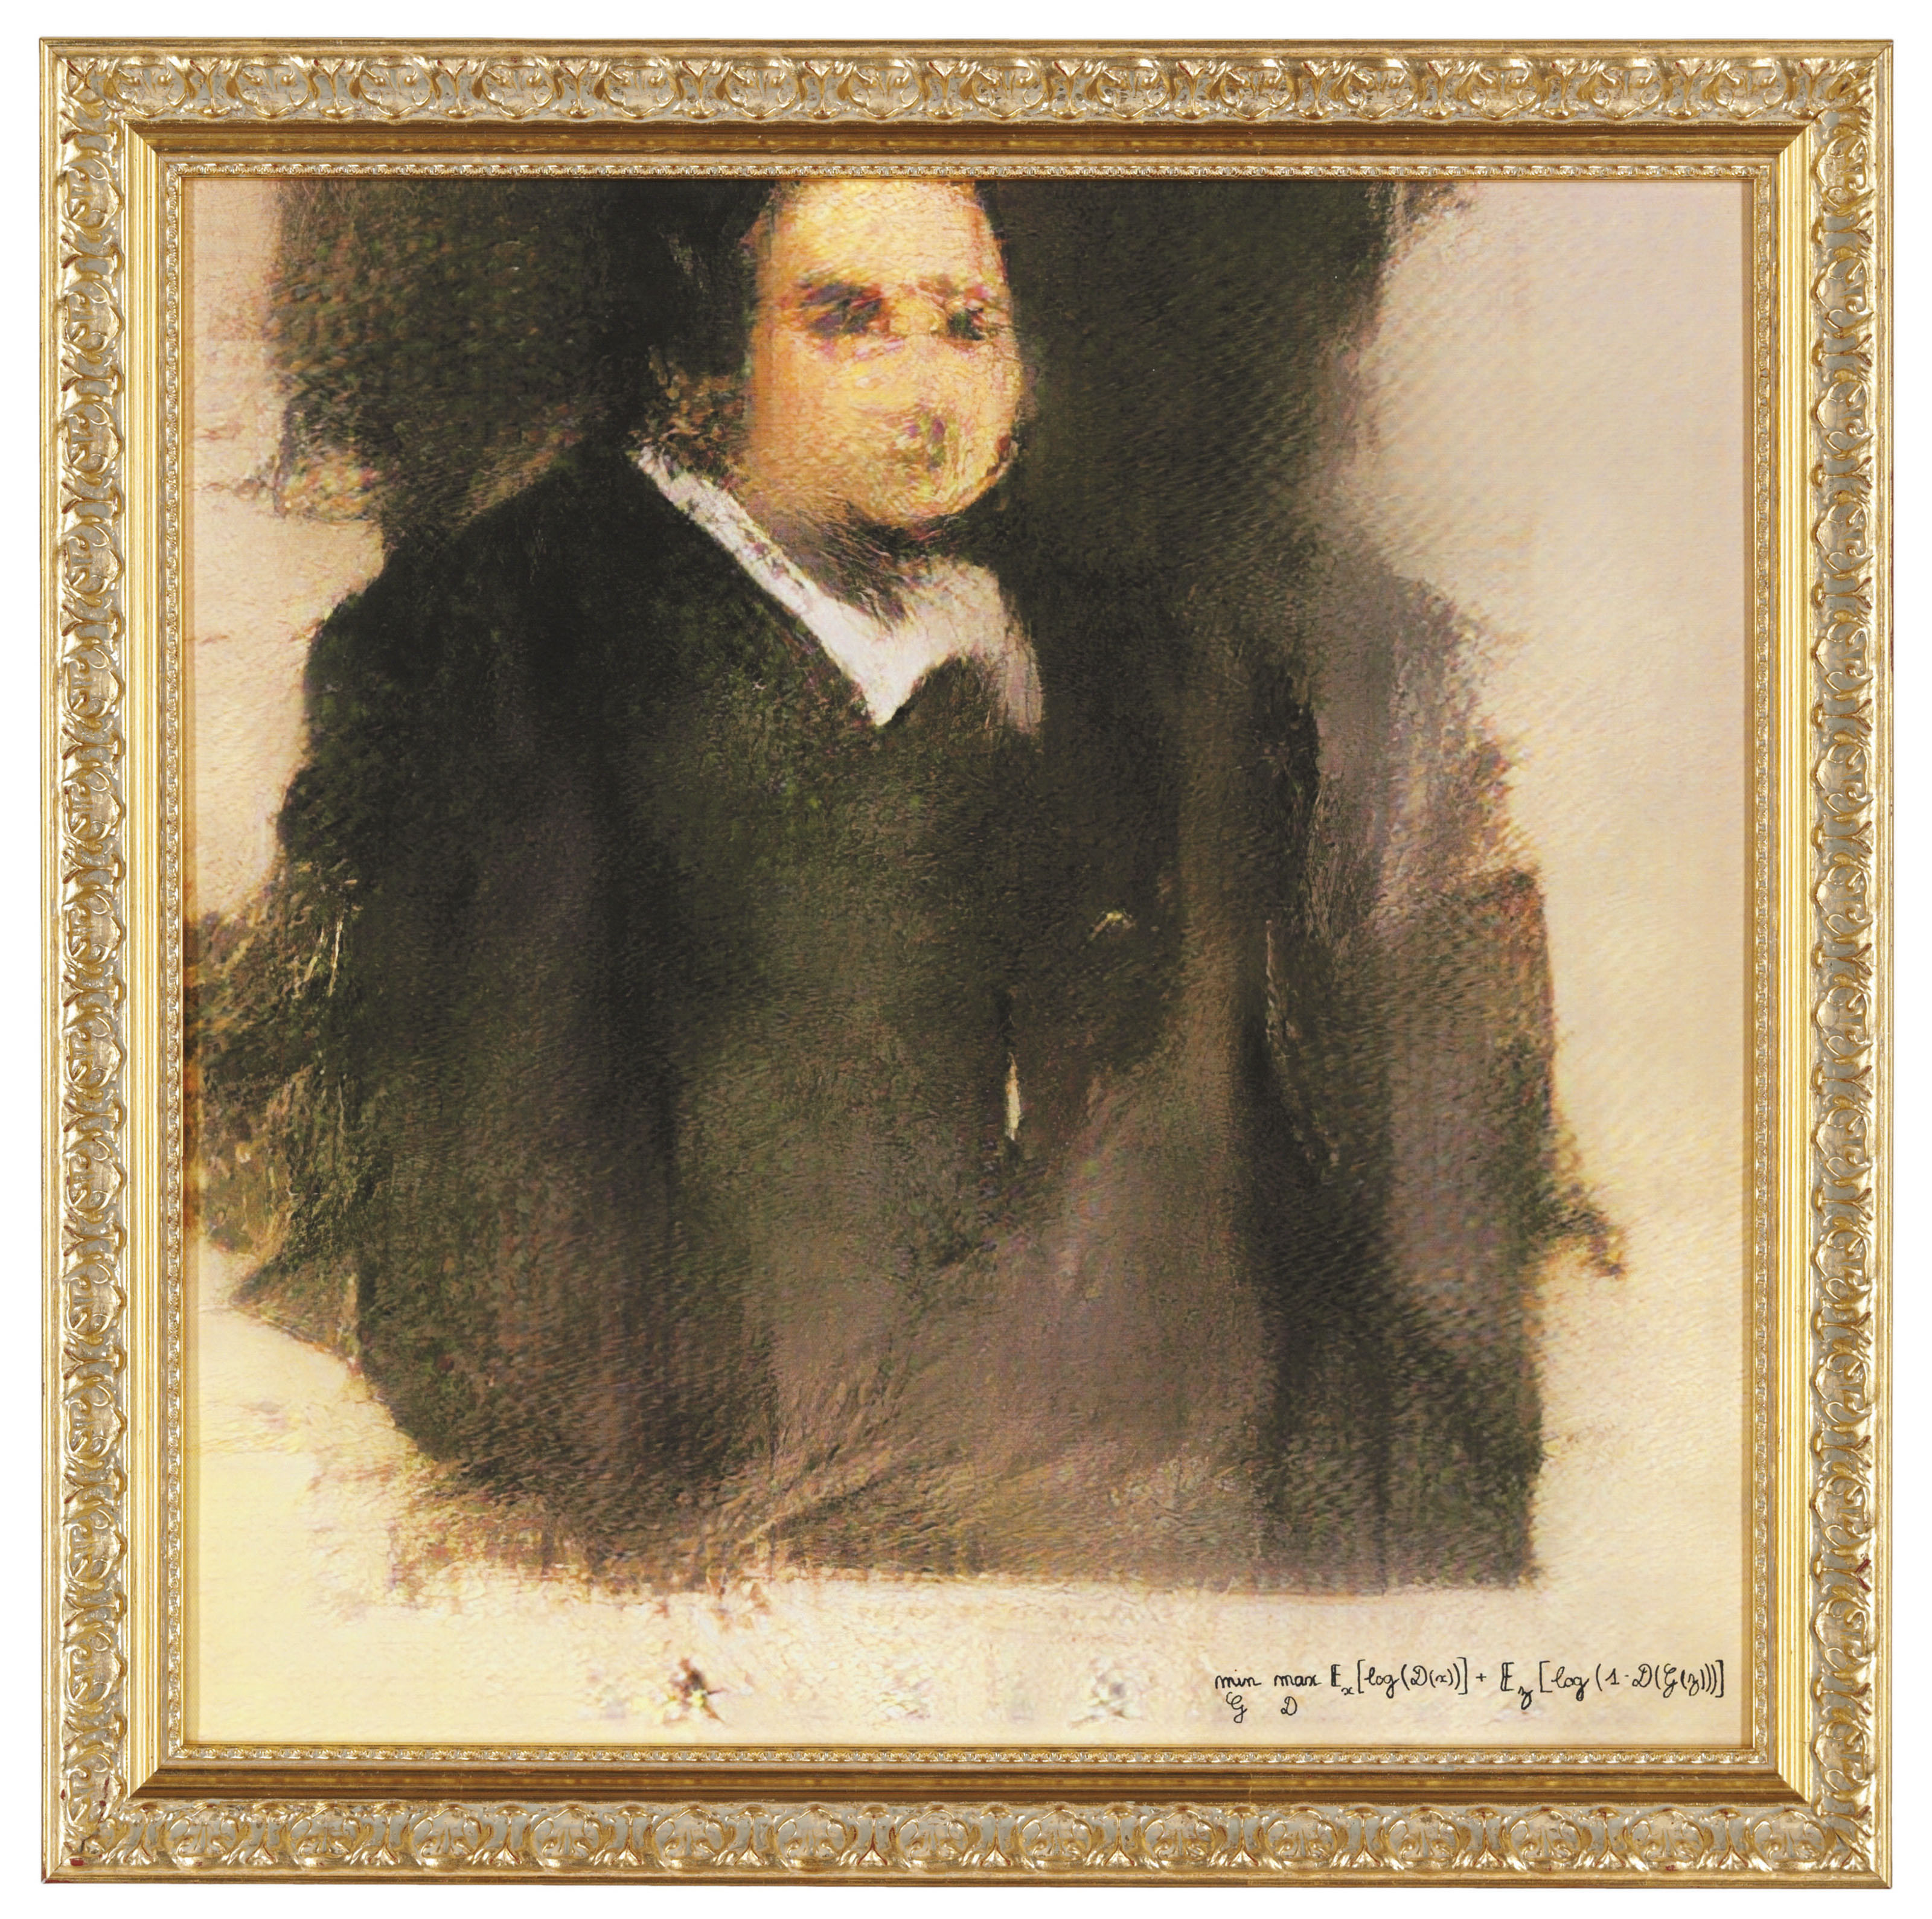
\includegraphics[width=0.6\textwidth]{../common/resources/portrait.jpg}
		\end{center}
		\caption{Portrait of Edmond Belamy \cite{Christies:PortraitEdmundBelamy}}
		\label{fig:Portrait of Edmond Belamy}
	\end{figure}

	\vspace{0.3\baselineskip} % Whitespace under the publisher logo

	2021 % Publication year

\end{titlepage}

    \newpage
    \tableofcontents

    \chapter{Einführung}
Am 25. Oktober 2018 wurde bei Christies das erste Gemälde verkauft, welches durch künstliche Intelligenz erschaffen
wurde \cite{Christies:PortraitEdmundBelamy}. Auf etwa 10'000 USD geschätzt, brachte es dem Anbieter doch über
432'500 USD ein. Es zeigt das Porträt einer fiktiven  Person namens Edmond Belamy,
trainiert mit über 15'000 Bildnissen verschiedener Epochen \cite{nzz:1:belamy}. Ob dieses \glqq Gemälde\grqq{} nun
als kreatives Werk angesehen werden kann, ist sehr umstritten und wird auch nicht weiter behandelt.
Es steht viel mehr der Künstler im Mittelpunkt. Der Künstler namens \Gls{GAN}.
\para
Doch wieso ist so ein \Gls{GAN} überhaupt von Interesse? Leser mit Vorkentnissen im Bereich der künstlichen neuronalen
Netzwerke haben wahrscheinlich schon gemerkt, dass es nicht trivial ist, neue Daten aufgrund von Bestehenden zu generieren.
Für alle, welche nicht Wissen, was gemeint ist, sei gesagt, dass ein \Gls{KNN} Daten klassifizieren kann, aber nicht unbedingt
neue Daten erzeugen. Das Generieren erfordert weitaus mehr.
Es soll ein kleines Beispiel behandelt werden, um aufzuzeigen, was gemeint ist. Die Idee zu diesem Gedankenexperiment
stammt von \glqq Computerphile\grqq{} \cite{youtube:gan}.
Ein neuronales Netz lernt auf Basis von Input-Daten ein Modell. In diesem Fall gibt es deren drei Input-Daten, welche in der Abbildung 1.1
dargestellt werden. Wie erkannt werden kann, sind diese Datenpunkte sehr zufällig gewählt.
\begin{figure}[h!]
    \begin{center}
        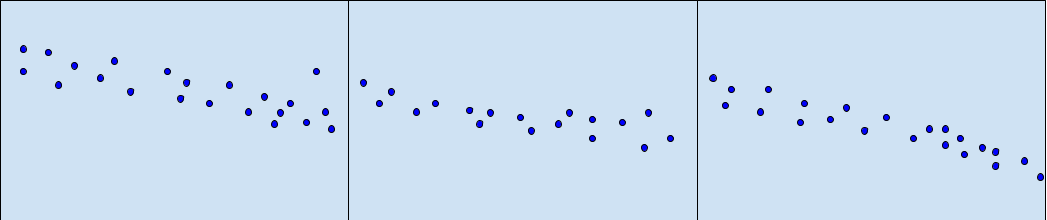
\includegraphics[width=0.6\textwidth]{../common/02_main/resources/00_input.png}
    \end{center}
    \caption{Input-Daten für \Gls{KNN}}
    \label{fig:Input-Daten für KNN}
\end{figure}
\newpage
Das Modell, welches das \Gls{KNN} lernt, kann wie in Abbildung 1.2 ersichtlich visualisiert werden. Es bildet eine möglichst
gute Annäherung an alle Datenpunkte ab.
\begin{figure}[h!]
    \begin{center}
        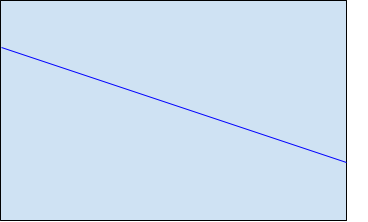
\includegraphics[width=0.4\textwidth]{../common/02_main/resources/01_modell.png}
    \end{center}
    \caption{Gelerntes Modell}
    \label{fig:Gelerntes Modell}
\end{figure}
Doch wie kann nun ein neues Sample, welches möglichst mit den Input-Daten korreliert, erzeugt werden? Das einzige, was
das Netzwerk wahrscheinlich kann, sind zufällige Datenpunkte auf der Modellgeraden bestimmen.
\begin{figure}[h!]
    \begin{center}
        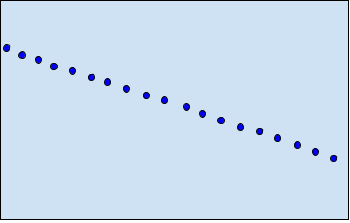
\includegraphics[width=0.4\textwidth]{../common/02_main/resources/02_generierte_punkte.png}
    \end{center}
    \caption{Generiertes Sample aufgrund von gelerntem Modell}
    \label{fig:Generiertes Sample aufgrund von gelerntem Modell}
\end{figure}
In der Abbildung 1.3 kann entnommen werden, dass dies nicht wirklich natürlich wirkt und nicht mit den Input-Daten übereinstimmt.
Die Frage stellt sich nun, wie also solche natürlich wirkenden Samples erzeugt werden können? Eine Antwort darauf liefert
\Gls{GAN}. Die vorliegende Arbeit geht der Fragestellung nach, wie diese \glqq Generative Adversarial Networks\grqq{}
funktionieren.
    \chapter{Einführung}
Am 25. Oktober 2018 wurde bei Christies das erste Gemälde verkauft, welches durch künstliche Intelligenz erschaffen
wurde \cite{Christies:PortraitEdmundBelamy}. Auf etwa 10'000 USD geschätzt, brachte es dem Anbieter doch über
432'500 USD ein. Es zeigt das Porträt einer fiktiven  Person namens Edmond Belamy,
trainiert mit über 15'000 Bildnissen verschiedener Epochen \cite{nzz:1:belamy}. Ob dieses \glqq Gemälde\grqq{} nun
als kreatives Werk angesehen werden kann, ist sehr umstritten und wird auch nicht weiter behandelt.
Es steht viel mehr der Künstler im Mittelpunkt. Der Künstler namens \Gls{GAN}.
\para
Doch wieso ist so ein \Gls{GAN} überhaupt von Interesse? Leser mit Vorkentnissen im Bereich der künstlichen neuronalen
Netzwerke haben wahrscheinlich schon gemerkt, dass es nicht trivial ist, neue Daten aufgrund von Bestehenden zu generieren.
Für alle, welche nicht Wissen, was gemeint ist, sei gesagt, dass ein \Gls{KNN} Daten klassifizieren kann, aber nicht unbedingt
neue Daten erzeugen. Das Generieren erfordert weitaus mehr.
Es soll ein kleines Beispiel behandelt werden, um aufzuzeigen, was gemeint ist. Die Idee zu diesem Gedankenexperiment
stammt von \glqq Computerphile\grqq{} \cite{youtube:gan}.
Ein neuronales Netz lernt auf Basis von Input-Daten ein Modell. In diesem Fall gibt es deren drei Input-Daten, welche in der Abbildung 1.1
dargestellt werden. Wie erkannt werden kann, sind diese Datenpunkte sehr zufällig gewählt.
\begin{figure}[h!]
    \begin{center}
        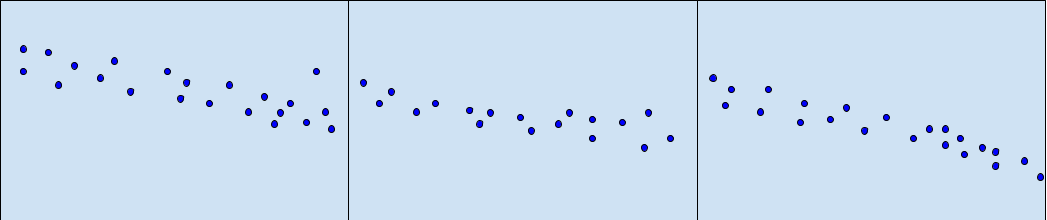
\includegraphics[width=0.6\textwidth]{../common/02_main/resources/00_input.png}
    \end{center}
    \caption{Input-Daten für \Gls{KNN}}
    \label{fig:Input-Daten für KNN}
\end{figure}
\newpage
Das Modell, welches das \Gls{KNN} lernt, kann wie in Abbildung 1.2 ersichtlich visualisiert werden. Es bildet eine möglichst
gute Annäherung an alle Datenpunkte ab.
\begin{figure}[h!]
    \begin{center}
        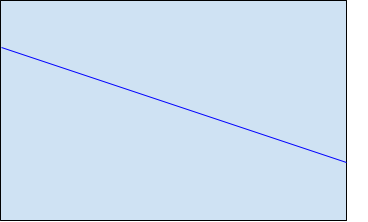
\includegraphics[width=0.4\textwidth]{../common/02_main/resources/01_modell.png}
    \end{center}
    \caption{Gelerntes Modell}
    \label{fig:Gelerntes Modell}
\end{figure}
Doch wie kann nun ein neues Sample, welches möglichst mit den Input-Daten korreliert, erzeugt werden? Das einzige, was
das Netzwerk wahrscheinlich kann, sind zufällige Datenpunkte auf der Modellgeraden bestimmen.
\begin{figure}[h!]
    \begin{center}
        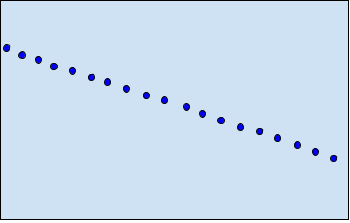
\includegraphics[width=0.4\textwidth]{../common/02_main/resources/02_generierte_punkte.png}
    \end{center}
    \caption{Generiertes Sample aufgrund von gelerntem Modell}
    \label{fig:Generiertes Sample aufgrund von gelerntem Modell}
\end{figure}
In der Abbildung 1.3 kann entnommen werden, dass dies nicht wirklich natürlich wirkt und nicht mit den Input-Daten übereinstimmt.
Die Frage stellt sich nun, wie also solche natürlich wirkenden Samples erzeugt werden können? Eine Antwort darauf liefert
\Gls{GAN}. Die vorliegende Arbeit geht der Fragestellung nach, wie diese \glqq Generative Adversarial Networks\grqq{}
funktionieren.
    \chapter{Einführung}
Am 25. Oktober 2018 wurde bei Christies das erste Gemälde verkauft, welches durch künstliche Intelligenz erschaffen
wurde \cite{Christies:PortraitEdmundBelamy}. Auf etwa 10'000 USD geschätzt, brachte es dem Anbieter doch über
432'500 USD ein. Es zeigt das Porträt einer fiktiven  Person namens Edmond Belamy,
trainiert mit über 15'000 Bildnissen verschiedener Epochen \cite{nzz:1:belamy}. Ob dieses \glqq Gemälde\grqq{} nun
als kreatives Werk angesehen werden kann, ist sehr umstritten und wird auch nicht weiter behandelt.
Es steht viel mehr der Künstler im Mittelpunkt. Der Künstler namens \Gls{GAN}.
\para
Doch wieso ist so ein \Gls{GAN} überhaupt von Interesse? Leser mit Vorkentnissen im Bereich der künstlichen neuronalen
Netzwerke haben wahrscheinlich schon gemerkt, dass es nicht trivial ist, neue Daten aufgrund von Bestehenden zu generieren.
Für alle, welche nicht Wissen, was gemeint ist, sei gesagt, dass ein \Gls{KNN} Daten klassifizieren kann, aber nicht unbedingt
neue Daten erzeugen. Das Generieren erfordert weitaus mehr.
Es soll ein kleines Beispiel behandelt werden, um aufzuzeigen, was gemeint ist. Die Idee zu diesem Gedankenexperiment
stammt von \glqq Computerphile\grqq{} \cite{youtube:gan}.
Ein neuronales Netz lernt auf Basis von Input-Daten ein Modell. In diesem Fall gibt es deren drei Input-Daten, welche in der Abbildung 1.1
dargestellt werden. Wie erkannt werden kann, sind diese Datenpunkte sehr zufällig gewählt.
\begin{figure}[h!]
    \begin{center}
        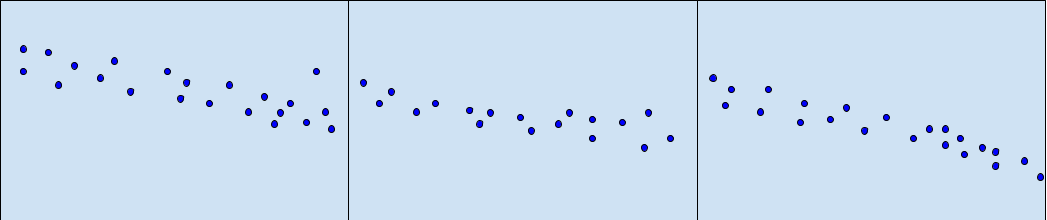
\includegraphics[width=0.6\textwidth]{../common/02_main/resources/00_input.png}
    \end{center}
    \caption{Input-Daten für \Gls{KNN}}
    \label{fig:Input-Daten für KNN}
\end{figure}
\newpage
Das Modell, welches das \Gls{KNN} lernt, kann wie in Abbildung 1.2 ersichtlich visualisiert werden. Es bildet eine möglichst
gute Annäherung an alle Datenpunkte ab.
\begin{figure}[h!]
    \begin{center}
        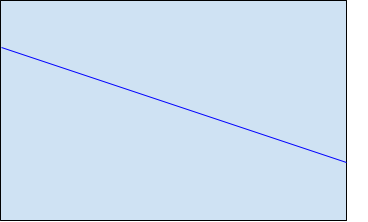
\includegraphics[width=0.4\textwidth]{../common/02_main/resources/01_modell.png}
    \end{center}
    \caption{Gelerntes Modell}
    \label{fig:Gelerntes Modell}
\end{figure}
Doch wie kann nun ein neues Sample, welches möglichst mit den Input-Daten korreliert, erzeugt werden? Das einzige, was
das Netzwerk wahrscheinlich kann, sind zufällige Datenpunkte auf der Modellgeraden bestimmen.
\begin{figure}[h!]
    \begin{center}
        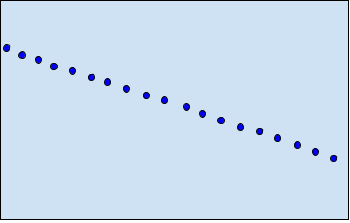
\includegraphics[width=0.4\textwidth]{../common/02_main/resources/02_generierte_punkte.png}
    \end{center}
    \caption{Generiertes Sample aufgrund von gelerntem Modell}
    \label{fig:Generiertes Sample aufgrund von gelerntem Modell}
\end{figure}
In der Abbildung 1.3 kann entnommen werden, dass dies nicht wirklich natürlich wirkt und nicht mit den Input-Daten übereinstimmt.
Die Frage stellt sich nun, wie also solche natürlich wirkenden Samples erzeugt werden können? Eine Antwort darauf liefert
\Gls{GAN}. Die vorliegende Arbeit geht der Fragestellung nach, wie diese \glqq Generative Adversarial Networks\grqq{}
funktionieren.
    \chapter{Einführung}
Am 25. Oktober 2018 wurde bei Christies das erste Gemälde verkauft, welches durch künstliche Intelligenz erschaffen
wurde \cite{Christies:PortraitEdmundBelamy}. Auf etwa 10'000 USD geschätzt, brachte es dem Anbieter doch über
432'500 USD ein. Es zeigt das Porträt einer fiktiven  Person namens Edmond Belamy,
trainiert mit über 15'000 Bildnissen verschiedener Epochen \cite{nzz:1:belamy}. Ob dieses \glqq Gemälde\grqq{} nun
als kreatives Werk angesehen werden kann, ist sehr umstritten und wird auch nicht weiter behandelt.
Es steht viel mehr der Künstler im Mittelpunkt. Der Künstler namens \Gls{GAN}.
\para
Doch wieso ist so ein \Gls{GAN} überhaupt von Interesse? Leser mit Vorkentnissen im Bereich der künstlichen neuronalen
Netzwerke haben wahrscheinlich schon gemerkt, dass es nicht trivial ist, neue Daten aufgrund von Bestehenden zu generieren.
Für alle, welche nicht Wissen, was gemeint ist, sei gesagt, dass ein \Gls{KNN} Daten klassifizieren kann, aber nicht unbedingt
neue Daten erzeugen. Das Generieren erfordert weitaus mehr.
Es soll ein kleines Beispiel behandelt werden, um aufzuzeigen, was gemeint ist. Die Idee zu diesem Gedankenexperiment
stammt von \glqq Computerphile\grqq{} \cite{youtube:gan}.
Ein neuronales Netz lernt auf Basis von Input-Daten ein Modell. In diesem Fall gibt es deren drei Input-Daten, welche in der Abbildung 1.1
dargestellt werden. Wie erkannt werden kann, sind diese Datenpunkte sehr zufällig gewählt.
\begin{figure}[h!]
    \begin{center}
        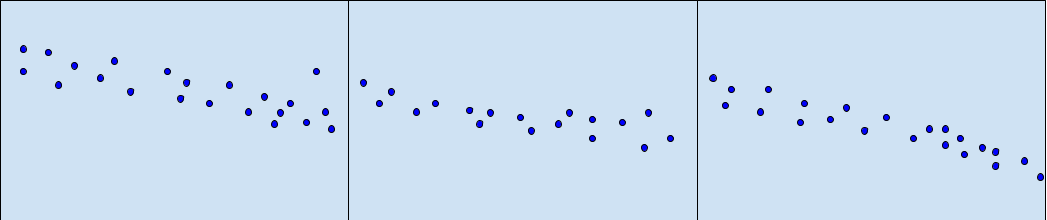
\includegraphics[width=0.6\textwidth]{../common/02_main/resources/00_input.png}
    \end{center}
    \caption{Input-Daten für \Gls{KNN}}
    \label{fig:Input-Daten für KNN}
\end{figure}
\newpage
Das Modell, welches das \Gls{KNN} lernt, kann wie in Abbildung 1.2 ersichtlich visualisiert werden. Es bildet eine möglichst
gute Annäherung an alle Datenpunkte ab.
\begin{figure}[h!]
    \begin{center}
        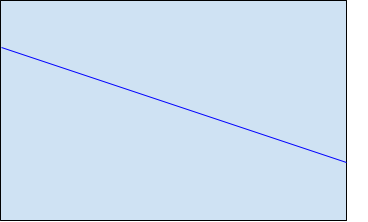
\includegraphics[width=0.4\textwidth]{../common/02_main/resources/01_modell.png}
    \end{center}
    \caption{Gelerntes Modell}
    \label{fig:Gelerntes Modell}
\end{figure}
Doch wie kann nun ein neues Sample, welches möglichst mit den Input-Daten korreliert, erzeugt werden? Das einzige, was
das Netzwerk wahrscheinlich kann, sind zufällige Datenpunkte auf der Modellgeraden bestimmen.
\begin{figure}[h!]
    \begin{center}
        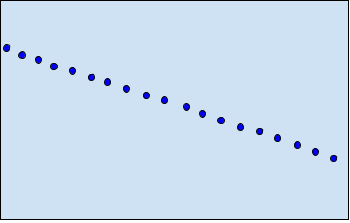
\includegraphics[width=0.4\textwidth]{../common/02_main/resources/02_generierte_punkte.png}
    \end{center}
    \caption{Generiertes Sample aufgrund von gelerntem Modell}
    \label{fig:Generiertes Sample aufgrund von gelerntem Modell}
\end{figure}
In der Abbildung 1.3 kann entnommen werden, dass dies nicht wirklich natürlich wirkt und nicht mit den Input-Daten übereinstimmt.
Die Frage stellt sich nun, wie also solche natürlich wirkenden Samples erzeugt werden können? Eine Antwort darauf liefert
\Gls{GAN}. Die vorliegende Arbeit geht der Fragestellung nach, wie diese \glqq Generative Adversarial Networks\grqq{}
funktionieren.

    \newpage
    \listoffigures
    \printbibliography[heading=bibintoc]
    \printunsrtglossary[style={index}]

\end{document}
